\documentclass[a4paper,10pt]{letter}
\usepackage[utf8]{inputenc}
\usepackage[spanish]{babel}
\usepackage[left=2cm, right=2cm, top=2cm, bottom=2cm]{geometry}
\usepackage{xcolor}
\usepackage{graphicx}
\usepackage{parskip}

\definecolor{darkblue}{rgb}{0.0, 0.0, 0.55}

\begin{document}

\begin{letter}{Comite de seleccion del "DIPLOMADO EN PRESERVACIÓN DEL PATRIMONIO SONORO, FOTOGRÁFICO Y AUDI€VISUAL"\\}

\opening{Estimado Comite seleccionador,}

Me dirijo a usted con el fin de expresar mi interés y motivación para participar en el Diplomado de Preservación de Archivos Sonoros que ofrece su prestigiosa institución. Mi nombre es Allan Ulises Zepeda Ibarra, y desde 2023 tengo el privilegio de formar parte de Música y Baile Tradicional A.C.

En mi papel como miembro de esta asociación, he tenido la responsabilidad de gestionar y preservar gran parte de nuestro invaluable archivo sonoro y audiovisual. Este material abarca desde 1995 hasta 2014 y constituye un testimonio vital de maestros de la tradición y fandangos campesinos de la región de la Tierra Caliente. Desafortunadamente, muchos de estos registros se encuentran en formatos antiguos como VHS, 8mm, minidisc, casete y algunos discos duros con fallas.

La situación actual de la sede de nuestra asociación, ubicada en un entorno rural con condiciones medioambientales desafiantes, presenta un riesgo significativo para la preservación de estos materiales en sus soportes originales. La exposición a condiciones climáticas extremas y la falta de recursos adecuados para el mantenimiento y la digitalización plantean amenazas inminentes para la integridad de nuestro archivo.

Mi participación en el diplomado no solo enriquecerá mis conocimientos en preservación de archivos sonoros, sino que también me capacitará para aplicar prácticas efectivas en el salvaguarda de nuestro valioso patrimonio cultural. Estoy convencido/a de que este programa proporcionará las herramientas y habilidades necesarias para enfrentar los desafíos específicos que enfrentamos en Música y Baile Tradicional A.C.

Agradezco la atención prestada y espero tener la oportunidad de contribuir al resguardo y difusión de nuestra rica herencia musical a través de la participación en este diplomado.



\closing{Atentamente\\ Allan Ulises Zepeda Ibarra}
\begin{center}
    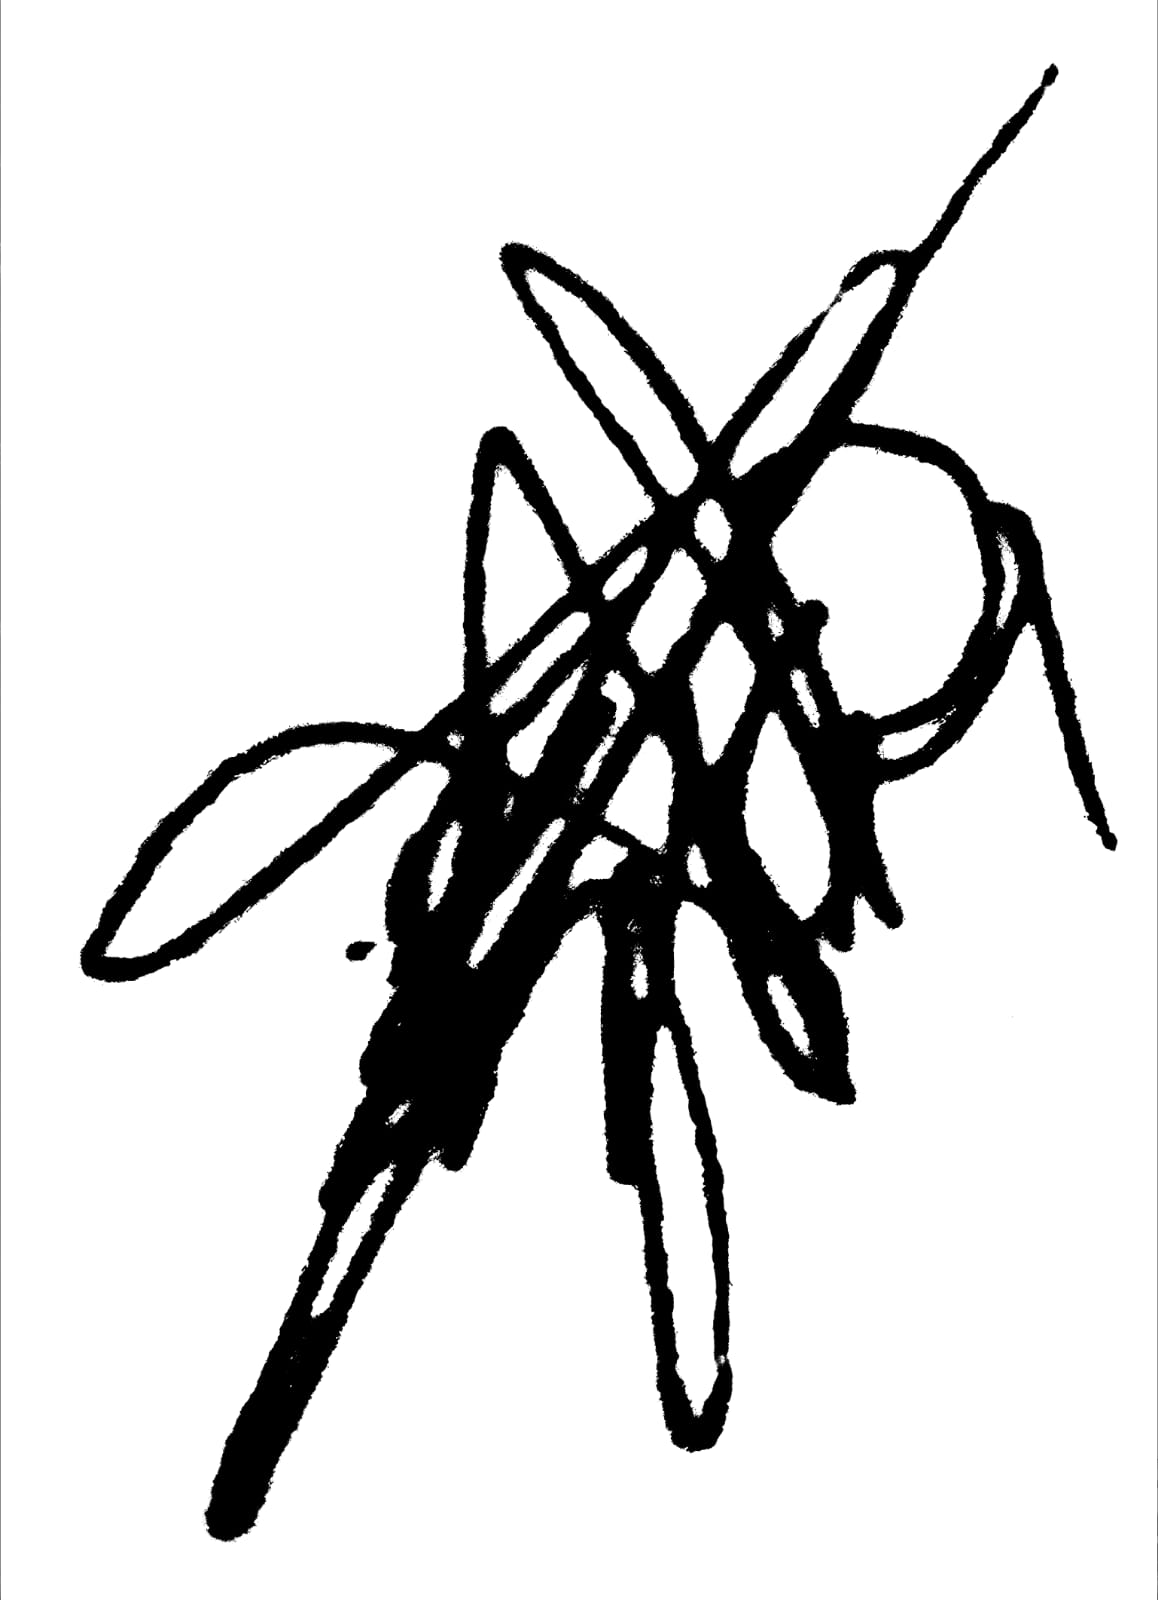
\includegraphics[width=2cm]{firma.png} % Asegúrate de reemplazar "firma.png" con el nombre de tu archivo de firma
  \end{center}

\end{letter}

\end{document}

